\documentclass[11pt]{article}

% "review" for submission (anonymous, line numbers), "final" for the camera-ready
% version, "preprint" for a non-anonymous version with page numbers.
\usepackage[review]{acl}

\usepackage{times}
\usepackage{latexsym}
\usepackage[T1]{fontenc}
\usepackage[utf8]{inputenc}
\usepackage{microtype}
\usepackage{inconsolata}
\usepackage{graphicx}
\usepackage{amsmath}
\usepackage{amssymb}
\usepackage{booktabs}
\usepackage{array}
\usepackage{multirow}
\usepackage{xcolor}
\usepackage{tikz}
\usetikzlibrary{positioning,arrows.meta,fit,calc}

% ---------------------------------------------------------------------------
% Draft markers. Red numbers are preliminary; --?-- marks results that are
% still missing. FG+PS and reproduced fine-tuned models in TAIL: mean over
% seeds 1-3 (with or without the alignment defect); noise ablations: seeds
% 1-2; HEAD runs and independent classifiers: one run each.
% Set \draftfalse once every number is final: the markers then disappear.
\newif\ifdraft
\draftfalse
\newcommand{\pend}[1]{\ifdraft\textcolor{red!75!black}{#1}\else#1\fi}
\newcommand{\tbd}{\ifdraft\textcolor{red!75!black}{--?--}\else--\fi}
\newcommand{\todo}[1]{\ifdraft\textcolor{blue!70!black}{[TODO: #1]}\fi}
% ---------------------------------------------------------------------------

\newcommand{\HEAD}{\textup{\textsc{Head}}}
\newcommand{\TAIL}{\textup{\textsc{Tail}}}
\newcommand{\sg}{\operatorname{sg}}
\newcommand{\JSD}{\operatorname{JSD}}
\newcommand{\CE}{\operatorname{CE}}
\newcommand{\tfidf}{TF$\ast$IDF}

% Repository link: hidden in the anonymous review version, shown with the final or preprint option.
\makeatletter
\newcommand{\repolink}{\ifacl@anonymize Link withheld for anonymous review.\else\url{https://github.com/Mano-08/rationalizing-neural-predictions}\fi}
\makeatother

\title{Freeze, Don't Perturb: Frozen Generators and Phrase Selection\\for Plausible Unsupervised Rationales}

\author{Mano W \and Maddili Gnana Pramod \and Hima Bindu Kommanti \\
  Department of Computer Science and Engineering \\
  National Institute of Technology, Andhra Pradesh, India \\
  \texttt{\{421215,421210\}@student.nitandhra.ac.in}, \texttt{himabinduk@nitandhra.ac.in}}

\begin{document}
\maketitle

\begin{abstract}
Unsupervised selective rationalization trains a generator to extract a rationale and a predictor to classify from it alone. Noise injection \citep{storek-etal-2023-unsupervised} replaces unimportant rationale words with random words during training and makes fine-tuned BERT generators more plausible. On USR Movie Review, it does not steer the generator: no gradient carries the noise back to the generator's choices, its selections are hit by noise as often as random ones, and every fine-tuned generator we trained selects more stopwords and punctuation than a random selection. Its benefit varies strongly between seeds, with or without a defect in the released code, and rationales are plausible only when the predictor no longer reads the label from which tokens are selected. Freezing the generator's encoder achieves this without noise; its rationales are more plausible on average than with noise injection and far more stable. Averaging attention over five-token windows to select phrases adds about three F1 points to every generator. The published numbers use the end of long reviews, the released code the beginning; on the end of each review, the two changes raise token F1 from 33.3 to 34.2, IOU-F1 from 38.4 to 50.9, and accuracy from 87.9 to 91.8.
\end{abstract}

% ===========================================================================
\section{Introduction}
% ===========================================================================

Selective rationalization makes a classifier inherently interpretable: a \emph{generator} extracts a short rationale from the input and a \emph{predictor} classifies from the extracted rationale alone \citep{lei-etal-2016-rationalizing}. Because the predictor never sees the rest of the input, the rationale is faithful to the prediction. Nothing in the training objective, however, asks the rationale to be \emph{plausible}, that is, to convince a human of the label \citep{jacovi-goldberg-2021-aligning}. Without rationale supervision, generator and predictor can agree on selections that predict the label without explaining it, such as stopwords and punctuation \citep{yu-etal-2019-rethinking}. Such a selection \emph{encodes} the label \citep{jethani-etal-2021-learned,puli-etal-2024-explanations}: the predictor reads the label from \emph{which} tokens are selected, not from their content. The problem grows with the capacity of the generator \citep{jacovi-goldberg-2021-aligning}.

\citet{storek-etal-2023-unsupervised} address this \emph{degeneration} with noise injection (NI): during training, words of the rationale with low \tfidf{} are replaced with random vocabulary words before the predictor reads them. They argue that the noise keeps the generator from learning how the predictor reads its selections, and report that with NI, a fine-tuned BERT generator \citep{devlin-etal-2019-bert} selects rationales closer to human ones than a frozen one on their USR Movie Review benchmark (token F1 33.3 vs.\ 30.0, IOU-F1 38.4 vs.\ 29.9).

We set out to improve NI by adapting the noise level during training. We could not, and this paper explains why and what works instead. In BERT-A2R, the architecture NI is applied to, the generator learns only from an \emph{attention-based predictor} that classifies the review from its attention. From the noisy rationale, it learns only the label guessed by the \emph{rationale-based predictor}, not which selected words were replaced (\S\ref{sec:analysis}). Accordingly, the words our generators select are hit by noise as often as randomly chosen words, and neither the published noise level ($p = 0.2$) nor a controller that adjusted it during training changed this. Every fine-tuned generator we trained also selected more stopwords and punctuation than a random selection.

Noise injection still makes a fine-tuned generator more plausible, by 2.4 to 8.1 F1 points in all four pairs of runs that share a seed and differ only in the noise. This is consistent with the noise breaking the encoding, but in two of three seeds the encoding survives the noise (\S\ref{sec:discussion}). The released code also has a defect: during training, it shows the rationale-based predictor the word before each selected word (App.~\ref{app:defects}). With this defect, NI \emph{as released} breaks the encoding in two of three seeds, but its plausibility varies almost as much as that of NI \emph{as described} (F1 23.3 to 32.5 vs.\ 19.5 to 31.4), and neither reaches the published 33.3 on average (\S\ref{sec:results}).

Finally, the published USR numbers correspond to an evaluation window that keeps the \emph{end} of each review (\TAIL), whereas the released code keeps the beginning (\HEAD; \S\ref{sec:protocol}). Because 85\% of the test reviews exceed BERT's 512-token limit, this choice alone changes F1 by 1.7 to 3.6 points.

The analysis points to the capacity of the generator rather than to the noise. We therefore keep the generator's encoder at its pretrained weights, so that only two linear layers are trained (2,307 parameters): the layer that scores each token to form the generator's attention and the classifier of the attention-based predictor. We also rank tokens by their attention averaged over a five-token window, so that the fixed number of tokens a rationale may contain is spent on phrases instead of isolated tokens (\S\ref{sec:method}). Neither change adds a training objective. Against our reproductions, the frozen generator is at least as plausible as NI as described in all three seeds and more plausible than the fine-tuned generator without noise. It is also more plausible than NI as released on average and varies far less between seeds. Phrase selection adds about three F1 points to every generator. In \TAIL, the window of the published numbers, the result improves on the best published model in IOU-F1 (50.9 vs.\ 38.4) and accuracy (91.8 vs.\ 87.9) and in token F1 by a margin that is not significant (34.2 vs.\ 33.3), and an epoch of its training takes about half as long as with a fine-tuned generator (\S\ref{sec:results}).

Our contributions are:
\begin{itemize}
  \setlength\itemsep{1pt}
  \item an analysis showing that noise injection does not steer the generator of BERT-A2R away from the words it replaces, with four diagnostics: the exposure of the selection to noise, its share of stopwords and punctuation, the accuracy of attention restricted to them, and the accuracy of the predictor on random selections;
  \item a reproducibility audit of the USR benchmark: a model-independent test that identifies the evaluation window from published precision and recall, and fixes for four defects in the released code, one of which changes the F1 of NI by $-4$ to $+10$ points;
  \item a frozen generator, which without any noise is more plausible on average than noise injection, as described or as released, and far more stable across seeds; and phrase selection, which adds about three F1 points to any generator; together they improve on the published state of the art on USR Movie Review under the published protocol;
  \item negative results for adaptive noise levels and for noise on the states that the attention-based predictor pools (evidence noise).
\end{itemize}
We release our code and all diagnostics.\footnote{\repolink}

% ===========================================================================
\section{Related Work}
% ===========================================================================

\paragraph{Selective rationalization.}
\citet{lei-etal-2016-rationalizing} train a generator and an encoder jointly with REINFORCE and penalties for sparsity and continuity. Later work makes selection differentiable \citep{bastings-etal-2019-interpretable}, maximizes the mutual information between the selected features and the model's output \citep{chen2018learning}, controls conciseness with an information bottleneck \citep{paranjape-etal-2020-information}, or frames rationalization as a game between several players \citep{chang2019game,chang2020invariant}. A2R \citep{yu2021understanding} adds an attention-based predictor that gives the generator a dense gradient, and BERT-A2R \citep{storek-etal-2023-unsupervised} replaces A2R's GloVe-based encoders with BERT: one BERT shared by the generator and the attention-based predictor, and a second one for the rationale-based predictor. Degeneration has been traced to the interplay of the two players: \citet{yu-etal-2019-rethinking} observe generators that communicate the label through punctuation, \citet{jacovi-goldberg-2021-aligning} argue that any generator able to represent the label can encode it in its selection, and \citet{zheng-etal-2022-irrationality} question how rational the rationale models are. Proposed remedies include a shared encoder \citep{liu2022fr}, a lower learning rate for the predictor \citep{liu2023dr}, multiple generators \citep{liu-etal-2023-mgr}, diagnostic objectives \citep{atanasova2022diagnostics}, and noise injection \citep{storek-etal-2023-unsupervised}. Where \citet{liu2023dr} slow down the predictor, we restrict the generator by freezing its encoder; on USR, the frozen generator is more plausible on average than a fine-tuned generator with noise injection (\S\ref{sec:results}). Supervised alternatives learn from annotated rationales \citep{zaidan-etal-2007-using,deyoung-etal-2020-eraser} or train the components separately \citep{jain-etal-2020-learning}; we stay unsupervised.

\paragraph{Contiguous rationales.}
Humans annotate phrases. Earlier models encourage contiguity with a fused-lasso penalty \citep{lei-etal-2016-rationalizing,bastings-etal-2019-interpretable}, structured inference \citep{guerreiro-martins-2021-spectra}, or by extracting contiguous spans \citep{jain-etal-2020-learning}. Our phrase selection is a parameter-free smoothing of the attention before top-$k$ selection and does not change the loss.

\paragraph{Frozen representations and attention.}
Frozen pretrained features are competitive with fine-tuning on many tasks \citep{peters-etal-2019-tune}, and a linear head on frozen states is a probe whose capacity is limited by design \citep{hewitt-liang-2019-designing}. Whether attention weights explain a model's predictions is debated \citep{jain-wallace-2019-attention,wiegreffe-pinter-2019-attention}; in selective rationalization the attention only decides what the predictor sees, so the rationale stays faithful.

\paragraph{Evaluation.}
We follow ERASER \citep{deyoung-etal-2020-eraser} for plausibility and faithfulness metrics and \citet{carton-etal-2020-evaluating} for normalized faithfulness; \citet{jacovi-goldberg-2020-towards} discuss the definitions. \citet{sun2019finetune} show that the part of a long review that BERT keeps affects its sentiment accuracy; we show that it also changes rationale metrics, so published numbers can only be compared within the same window. Our check of the released code and the published numbers adds to research on reproducibility in NLP \citep{belz-etal-2021-systematic}.

% ===========================================================================
\section{Background: BERT-A2R with Noise Injection}
\label{sec:background}
% ===========================================================================

Let $x = (x_1, \dots, x_T)$ be a tokenized review with label $y$. BERT-A2R \citep{storek-etal-2023-unsupervised} has three parts (Figure~\ref{fig:architecture}).

\paragraph{Generator.} A BERT encoder maps $x$ to states $h_1, \dots, h_T$. A linear scorer computes $s_i = w^\top h_i$, and $a = \operatorname{softmax}(s)$ is the generator's attention.

\paragraph{Attention-based predictor.} It shares the generator's encoder and classifies from the attention-pooled states, which we call its \emph{evidence}: $\hat{y}^a = \operatorname{softmax}(W \sum_i a_i h_i)$.

\paragraph{Selection and rationale-based predictor.} The rationale mask $m$ keeps the $k = \operatorname{round}(0.2\,T)$ tokens with the highest attention. A second BERT reads the selected tokens in their original order and predicts $\hat{y}^r$.

\paragraph{Training.} Each predictor minimizes its cross-entropy (CE) plus a closeness term, the Jensen--Shannon divergence (JSD) to the other predictor:
\begin{align}
  \mathcal{L}_a &= \CE(\hat{y}^a, y) + \lambda \JSD\big(\hat{y}^a, \sg[\hat{y}^r]\big), \label{eq:la} \\
  \mathcal{L}_r &= \CE(\hat{y}^r, y) + \lambda \JSD\big(\sg[\hat{y}^a], \hat{y}^r\big), \label{eq:lr}
\end{align}
where $\sg$ stops the gradient and $\lambda = 0.1$. The generator receives gradient only from Eq.~\ref{eq:la}: top-$k$ selection passes no gradient, and $\sg$ blocks the path through the attention-based predictor in Eq.~\ref{eq:lr}. As in the released code, the implementation differs from Eqs.~\ref{eq:la}--\ref{eq:lr} in details that affect all models alike (App.~\ref{app:defects}).

\paragraph{Noise injection.} During training, each selected word $x_i$ is replaced with probability $\min(1, p\,r_i)$ before the rationale-based predictor reads it, a scheme adapted from unsupervised data augmentation \citep{xie2020uda}. The replacement is drawn from the vocabulary with a probability that decreases with its ATF$\ast$IDF (\tfidf{} with the term frequency averaged over the corpus), to avoid drawing words that indicate a label. The replacement weight
\begin{equation}
  r_i = |d| \, \frac{t_{\max} - t_i}{\sum_{j \in d} (t_{\max} - t_j)}
  \label{eq:r}
\end{equation}
is high for words with low \tfidf{} $t_i$ in document $d$, where $t_{\max}$ is the highest \tfidf{} in $d$. By construction, $r$ has mean 1 over a document, so a randomly selected word is replaced with probability $p$ on average. \citet{storek-etal-2023-unsupervised} use $p = 0.2$ on USR.

\paragraph{Names.} A2R denotes our reproduction of BERT-A2R with a fine-tuned generator and no noise, not the GloVe-based A2R of \citet{yu2021understanding}. A2R+NI, or +NI, adds NI as described, and +NI\textsubscript{released} adds NI as released (App.~\ref{app:defects}). FG is our frozen generator and PS our phrase selection (\S\ref{sec:method}). \HEAD{} and \TAIL{} are the evaluation windows that keep the beginning and the end of reviews longer than 512 wordpieces (\S\ref{sec:protocol}). \S\ref{sec:setup} lists all models.

\begin{figure*}[t]
\centering
\resizebox{\textwidth}{!}{%
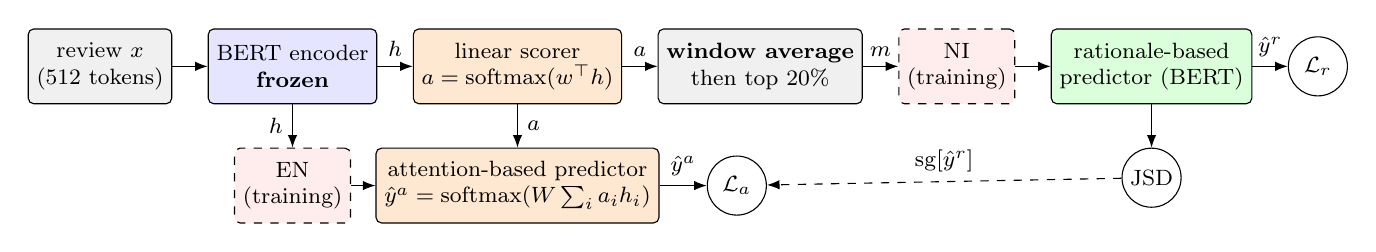
\begin{tikzpicture}[
  font=\footnotesize,
  box/.style={draw, rounded corners=2pt, align=center, minimum height=0.95cm, inner sep=3pt},
  frozen/.style={box, fill=blue!10},
  gen/.style={box, fill=orange!18},
  pred/.style={box, fill=green!14},
  fixed/.style={box, fill=gray!12},
  noise/.style={box, dashed, fill=red!7},
  loss/.style={draw, circle, inner sep=1pt, minimum size=0.75cm, fill=white},
  arr/.style={-{Latex[length=1.6mm]}},
  node distance=0.55cm and 0.45cm]
  \node[fixed] (x) {review $x$\\(512 tokens)};
  \node[frozen, right=of x] (enc) {BERT encoder\\\textbf{frozen}};
  \node[gen, right=of enc] (scorer) {linear scorer\\$a = \operatorname{softmax}(w^\top h)$};
  \node[fixed, right=of scorer] (sel) {\textbf{window average}\\then top 20\%};
  \node[noise, right=of sel] (ni) {NI\\(training)};
  \node[pred, right=of ni] (rp) {rationale-based\\predictor (BERT)};
  \node[loss, right=of rp] (lr) {$\mathcal{L}_r$};
  \node[gen, below=of scorer] (ap) {attention-based predictor\\$\hat{y}^a = \operatorname{softmax}(W \sum_i a_i h_i)$};
  \node[noise, below=of enc] (en) {EN\\(training)};
  \node[loss, right=0.6cm of ap] (la) {$\mathcal{L}_a$};
  \node[loss, below=of rp] (jsd) {JSD};
  \draw[arr] (x) -- (enc);
  \draw[arr] (enc) -- node[above] {$h$} (scorer);
  \draw[arr] (scorer) -- node[above] {$a$} (sel);
  \draw[arr] (sel) -- node[above] {$m$} (ni);
  \draw[arr] (ni) -- (rp);
  \draw[arr] (rp) -- node[above] {$\hat{y}^r$} (lr);
  \draw[arr] (enc) -- node[left] {$h$} (en);
  \draw[arr] (en) -- (ap);
  \draw[arr] (scorer) -- node[right] {$a$} (ap);
  \draw[arr] (ap) -- node[above] {$\hat{y}^a$} (la);
  \draw[arr] (rp) -- (jsd);
  \draw[arr, dashed] (jsd) -- node[above] {$\operatorname{sg}[\hat{y}^r]$} (la);
\end{tikzpicture}}
\caption{BERT-A2R and our changes (bold). Orange: the generator, trained only by $\mathcal{L}_a$ (Eq.~\ref{eq:la}); green: the rationale-based predictor, trained by $\mathcal{L}_r$; blue: frozen in our model. The rationale-based predictor reaches $\mathcal{L}_a$ only through a stop-gradient JSD term (dashed), and top-$k$ selection passes no gradient, so noise on the rationale (NI) cannot tell the generator which selected word was replaced. Noise on the generator's evidence (EN, \S\ref{sec:en}) enters $\mathcal{L}_a$ directly. We freeze the encoder and average the attention over a window before selection.}
\label{fig:architecture}
\end{figure*}

% ===========================================================================
\section{What Noise Injection Does Not Do}
\label{sec:analysis}
% ===========================================================================

\subsection{No token-level credit assignment}
\label{sec:credit}

Since only Eq.~\ref{eq:la} reaches the generator (\S\ref{sec:background}), the rationale-based predictor affects it only through $\sg[\hat{y}^r]$, a two-class distribution for the whole document weighted by $\lambda = 0.1$. When noise replaces a selected word, the generator can therefore learn at most that $\hat{y}^r$ changed, not which word was replaced or that selecting it was a mistake. The mechanism NI relies on, making implausible selections costly for the generator, has no path in this architecture.

This gives a simple test. If NI punished the generator for selecting the words it tends to replace, the generator would learn to stop selecting them. We measure this with the \emph{exposure} of a rationale: the average replacement weight $r_i$ (Eq.~\ref{eq:r}) of its words. Because $r$ averages 1 over a review, a random selection has an exposure of about 1; a selection that avoids the words NI tends to replace has a lower exposure, and one that prefers them a higher one. In every run with NI, the exposure stays at about 1.0 throughout training (1.02 at the end of training in both seeds of the frozen generator of \S\ref{sec:method} with NI, and 1.02--1.08 in the three seeds of the fine-tuned generator trained in \TAIL). The generator never learns to avoid the noise: its words are replaced at least as often as randomly chosen ones.

\subsection{Fine-tuned generators select stopwords and punctuation}
\label{sec:degeneration}

\begin{table}[t]
\centering
\small
\setlength{\tabcolsep}{4pt}
\begin{tabular}{@{}lcccccc@{}}
\toprule
Model & Acc & P & R & F1 & IOU & Stop \\
\midrule
\multicolumn{7}{@{}l}{\emph{Fine-tuned generator, trained in \HEAD}} \\
A2R & 88.1 & 11.2 & 30.6 & 16.4 & 17.8 & .64 \\
\ + NI & 85.1 & 13.4 & 36.7 & 19.6 & 20.5 & .56 \\
\ + NI\textsubscript{released} & 81.7 & 16.8 & 46.1 & 24.7 & 27.3 & .61 \\
\ + NI\textsubscript{PI} & 81.3 & 11.6 & 31.8 & 17.0 & 17.5 & .71 \\
\midrule
\multicolumn{7}{@{}l}{\emph{Fine-tuned generator, trained in \TAIL}} \\
A2R & 86.4 & 12.1 & 33.1 & 17.7 & 17.6 & .65 \\
\ + NI & 85.0 & 14.7 & 40.1 & 21.5 & 24.0 & .63 \\
\ + NI\textsubscript{released} & 84.7 & 16.8 & 45.8 & 24.5 & 27.6 & .63 \\
\midrule
\multicolumn{7}{@{}l}{\emph{Frozen generator, trained in \TAIL}} \\
FG & 87.1 & 19.0 & 52.0 & 27.8 & 27.0 & .41 \\
FG + PS & 88.4 & 21.1 & 57.8 & \textbf{31.0} & \textbf{46.8} & .51\textsuperscript{$\ast$} \\
\midrule
Random selection & -- & 7.3 & 20.0 & 10.7 & -- & .51 \\
Human rationales & -- & -- & -- & -- & -- & .46 \\
\bottomrule
\end{tabular}
\caption{Evaluation in \HEAD, the window of the released code, which keeps the beginning of each review (\S\ref{sec:protocol}; runs trained in \HEAD: seed 1; runs trained in \TAIL{} and evaluated here in \HEAD: mean over three seeds). Stop: share of stopwords and punctuation among the selected words. NI\textsubscript{released}: NI with the alignment defect of the released code (App.~\ref{app:defects}); NI\textsubscript{PI}: noise level set by a controller on predictor disagreement. FG: frozen generator; PS: phrase selection (\S\ref{sec:method}). Random selection: expected scores of selecting 20\% of the tokens at random; its share of stopwords and punctuation is measured on random selections in \TAIL. Human rationales: all annotated words of the test reviews. \textsuperscript{$\ast$}Phrases include the stopwords and punctuation between content words, as human rationales do.}
\label{tab:degeneration}
\end{table}

Table~\ref{tab:degeneration} shows our reproduction of BERT-A2R with a fine-tuned generator under the protocol of the released code. Trained in \HEAD, it reaches token F1 between 16.4 and 24.7 across noise settings, and every run spends more of its rationale on stopwords and punctuation (56--71\%) than a random selection of the same size (51\%), the human annotators (46\%), or a frozen generator (41\%). NI as described raises F1 from 16.4 to 19.6 in this single seed without lowering the exposure; NI as released, whose rationale-based predictor receives the token \emph{before} each selected token (App.~\ref{app:defects}), reaches 24.7. A closed-loop controller that raised $p$ whenever the two predictors disagreed on the clean rationale had nothing to react to: they agreed even when 71\% of the rationale was stopwords and punctuation. Even the two runs trained in \TAIL{} that come close to the published results spend 63\% and 56\% of their selections on stopwords and punctuation (\S\ref{sec:results}).

\subsection{A contextual encoder can place the label on any token}
\label{sec:anywhere}

Why does the generator not prefer the words that express the sentiment? Its only objective, Eq.~\ref{eq:la}, asks the attention-pooled states to predict the label. Each state of a deep contextual encoder mixes information from the whole review, so the label is available at almost any position. We verify this with generator heads trained on cached BERT-base states (App.~\ref{app:diagnostics}): restricting the attention to stopwords and punctuation leaves accuracy almost unchanged, both for pretrained states (83.2\% vs.\ 83.7\% with free attention) and for the states of a BERT fine-tuned on IMDb (90.3\% vs.\ 90.6\%). A fine-tuned scorer can also encode the label in \emph{which} tokens it selects. To show this, we let the scorer read fine-tuned states but give the attention-based predictor BERT's input (layer-0) embeddings as evidence and allow attention only on stopwords and punctuation. Layer-0 embeddings depend only on a token and its position, not on the rest of the review, so these tokens carry no sentiment there. The predictor still reaches 89.5\% accuracy, against 61.1\% when the scorer reads layer-0 embeddings as well and so chooses without seeing the rest of the review: the label is carried by which stopwords and punctuation marks the fine-tuned scorer chooses. This is the encoding that \citet{yu-etal-2019-rethinking} and \citet{jacovi-goldberg-2021-aligning} describe. Rationale noise does not reach the place where the encoding is formed; at most, it keeps the predictor from reading it (\S\ref{sec:discussion}). Even noise that does reach the generator (evidence noise, \S\ref{sec:en}) does not help a fine-tuned encoder (App.~\ref{app:diagnostics}). What a fine-tuned generator selects depends on its capacity to encode the label, which motivates freezing it.

% ===========================================================================
\section{Method}
\label{sec:method}
% ===========================================================================

\subsection{Frozen generator (FG)}

We keep the generator's encoder at its pretrained BERT-base weights and train only the scorer $w$ and the classifier $W$ of the attention-based predictor ($769 + 1{,}538 = 2{,}307$ parameters). The rationale-based predictor is fine-tuned as before, and the losses (Eqs.~\ref{eq:la}--\ref{eq:lr}) are unchanged. With frozen states, the scorer is a linear probe \citep{hewitt-liang-2019-designing}: it ranks tokens along one direction of a fixed representation space and has far less freedom to encode the label than a fine-tuned encoder. Empirically, it prefers content words: on average, only 41\% (\HEAD, Table~\ref{tab:degeneration}) and 42\% (\TAIL) of its single-token selections are stopwords and punctuation, fewer than in a random selection (51\%) or in human rationales (46\%). \citet{storek-etal-2023-unsupervised} report this configuration as their fixed-generator baseline; with matched evaluation, it is more plausible on average than our reproductions of their best model, the fine-tuned generator with NI, with or without the defect of the released code (\S\ref{sec:results}).

\subsection{Phrase selection (PS)}

Top-$k$ selection of single tokens produces scattered tokens: the frozen generator's selections form spans of 1.9 words on average, while human rationales consist of spans of 7.7 words. We rank tokens by their attention averaged over a centered window of $w$ tokens,
\begin{equation}
  \tilde{a}_i = \frac{1}{|N_i|} \sum_{j \in N_i} a_j,
  \label{eq:window}
\end{equation}
where $N_i = \{ j : |j - i| \le (w-1)/2,\ 1 \le j \le T \}$, and select the $k$ tokens with the highest $\tilde{a}_i$. The budget $k$ is unchanged. A token with high attention lifts its neighbors, so the budget is spent on phrases around the tokens the generator ranks highest. Phrase selection has no parameters, is applied in the same way during training and evaluation, and can be applied to any trained generator. We use $w = 5$, shorter than the average human span; \S\ref{sec:ablations} reports $w \in \{1, 5, 9\}$.

\subsection{Evidence noise (EN), a diagnostic variant}
\label{sec:en}

NI cannot reach the generator (\S\ref{sec:credit}). To test whether noise helps once it can, we move it into the evidence of the attention-based predictor, whose loss $\mathcal{L}_a$ does reach the generator. During training, each state $h_i$ in the sum $\sum_i a_i h_i$ is replaced, with probability $\min(1, p\,r_i)$, by the state of a random word from the batch; no gradient flows into this replacement state. The attention $a$ is still computed from the clean states. If the generator attends to a word that the noise tends to replace, the predictor sees an unreliable state, its loss $\mathcal{L}_a$ rises, and the gradient tells the generator to attend to that word less. We measure the effect with the \emph{attention exposure} $E = \sum_i a_i r_i$, the attention-weighted average of $r$: it is about 1 for uniform attention and lower if the attention avoids the words the noise tends to replace. We also tried a proportional-integral controller that adjusts $p$ during training to hold $E$ at a target (App.~\ref{app:noise}).

% ===========================================================================
\section{Experimental Setup}
\label{sec:setup}
% ===========================================================================

\paragraph{Data.}
USR Movie Review \citep{storek-etal-2023-unsupervised} trains on 40,000 IMDb reviews \citep{maas-etal-2011-learning}, validates on 10,000 more, and tests on the 2,000 reviews of ERASER Movie Reviews \citep{deyoung-etal-2020-eraser,zaidan-eisner-2008-modeling,pang-lee-2004-sentimental}, which carry token-level human rationales. The test reviews are long (774 words on average), and 85\% of them exceed 512 wordpieces. Human rationales cover 7.6\% of the words, in 7.6 spans of 7.7 words per review; 46\% of their words are stopwords and punctuation.

\paragraph{Evaluation window.}
\label{sec:protocol}
For a review longer than 512 wordpieces, BERT sees either its beginning (\HEAD, the released code) or its end (\TAIL). The choice matters for plausibility: 54\% of the human-annotated words survive truncation in \HEAD{} and 68\% in \TAIL, presumably because reviewers often state their verdict at the end. Which window do the published numbers use? Every model selects the same fraction of the tokens. Micro precision $P = \mathrm{TP}/S$ and recall $R = \mathrm{TP}/G$ share their numerator, the number TP of selected tokens that are annotated, so their ratio $R/P = S/G$, the number $S$ of selected tokens divided by the number $G$ of annotated tokens inside the window, is a property of the window, not of the model. All our evaluations give $R/P = 2.735$ in \HEAD{} and $2.164$--$2.165$ in \TAIL; all four USR rows of \citet{storek-etal-2023-unsupervised} give $2.16$ (App.~\ref{app:window}). The published numbers therefore correspond to \TAIL, and we compare with them in \TAIL{} only, reporting \HEAD{} as well. As in the released code, plausibility is computed over the tokens inside the window.

\paragraph{Metrics.}
\emph{Plausibility}: following \citet{storek-etal-2023-unsupervised}, token-level micro precision, recall and F1 against the human rationales, and IOU-F1 with partial-match threshold 0.1 \citep{deyoung-etal-2020-eraser,paranjape-etal-2020-information}. \emph{Accuracy}: of the rationale-based predictor. \emph{Faithfulness}: comprehensiveness and sufficiency \citep{deyoung-etal-2020-eraser} of the rationale-based predictor, on the sigmoid scale of the released code (for comparability) and on actual probabilities. Because a predictor trained on rationales is out of distribution on full reviews, we also score faithfulness with an independent BERT classifier trained on full reviews, raw and normalized by the empty input \citep{carton-etal-2020-evaluating}, and as the area over the perturbation curve (AOPC) \citep{deyoung-etal-2020-eraser}. \emph{Diagnostics}: a random selection of the same size, the share of stopwords and punctuation among the selected words, and the mean span length. App.~\ref{app:definitions} details how every reported quantity is computed.

\paragraph{Models.}
\emph{Published:} the four BERT-A2R variants of \citet{storek-etal-2023-unsupervised} (fixed or fine-tuned generator, with or without NI). \emph{Reproduced:} BERT-A2R with a fine-tuned generator without noise (A2R), with NI at $p = 0.2$ as described, i.e.\ after fixing the alignment defect (+NI), with NI as released (+NI\textsubscript{released}), and with NI whose level is set by a controller on predictor disagreement (+NI\textsubscript{PI}), all trained in \HEAD{} with seed 1; A2R, +NI and +NI\textsubscript{released} are also trained in \TAIL{} with seeds 1 to 3. \emph{Ours:} the frozen generator with phrase selection (FG+PS), the same model evaluated with single tokens (FG), and FG+PS trained with noise on the rationale (+NI, $p = 0.2$) or on the evidence (+EN, $p = 0.3$).

\paragraph{Implementation.}
We use \texttt{bert-base-uncased} with Transformers \citep{wolf-etal-2020-transformers} and the settings of \citet{storek-etal-2023-unsupervised}: Adam \citep{kingma2015adam} with learning rate $2 \cdot 10^{-5}$ for both components, batch size 16, at most 5 epochs, $k = 20\%$ and $\lambda = 0.1$. We keep the checkpoint of the last epoch in which both validation losses improved (patience 2); validation is noise-free. Unlike \citet{storek-etal-2023-unsupervised}, who train the fixed generator with batch size 64 for 10 epochs, we use the same settings for all models. Each run uses one NVIDIA T4 GPU (16 GB). We report FG+PS and the fine-tuned models trained in \TAIL{} as means over three seeds and the noise variants of FG+PS over seeds 1 and 2. Differences are computed from unrounded means. Same-seed models are compared with a paired bootstrap, and faithfulness is also scored by an independent BERT classifier (App.~\ref{app:training}).

% ===========================================================================
\section{Results}
\label{sec:results}
% ===========================================================================

\begin{table}[t]
\centering
\small
\setlength{\tabcolsep}{3.2pt}
\begin{tabular}{@{}lccccc@{}}
\toprule
Model & Acc & P & R & F1 & IOU \\
\midrule
\multicolumn{6}{@{}l}{\emph{Published \citep{storek-etal-2023-unsupervised}, 5 seeds}} \\
Fixed gen. & 85.0\textsubscript{0.8} & 21.9 & 47.4 & 30.0\textsubscript{0.5} & 29.9\textsubscript{0.6} \\
Fixed gen.\ + NI & 85.8\textsubscript{1.1} & 22.3 & 48.2 & 30.5\textsubscript{0.6} & 30.7\textsubscript{0.8} \\
Tuned gen. & 82.4\textsubscript{8.6} & 20.2 & 43.7 & 27.6\textsubscript{3.0} & 29.1\textsubscript{5.3} \\
Tuned gen.\ + NI & 87.9\textsubscript{1.8} & 24.4 & 52.7 & 33.3\textsubscript{0.8} & 38.4\textsubscript{1.9} \\
\midrule
\multicolumn{6}{@{}l}{\emph{Reproduced, tuned generator, trained in \TAIL}} \\
A2R & 89.1\textsubscript{1.8} & 14.2 & 30.7 & 19.4\textsubscript{3.4} & 19.0\textsubscript{2.8} \\
\ + PS\textsuperscript{$\ddagger$} & 80.3\textsubscript{12.2} & 16.4 & 35.5 & 22.4\textsubscript{2.5} & 33.9\textsubscript{3.5} \\
\ + NI & 88.6\textsubscript{3.4} & 17.9 & 38.8 & 24.5\textsubscript{6.2} & 27.1\textsubscript{7.2} \\
\ + NI + PS\textsuperscript{$\ddagger$} & 86.4\textsubscript{5.0} & 19.8 & 42.8 & 27.0\textsubscript{6.7} & 41.4\textsubscript{9.8} \\
\ + NI\textsubscript{released} & 87.1\textsubscript{4.4} & 20.2 & 43.7 & 27.6\textsubscript{4.6} & 30.9\textsubscript{4.8} \\
\ + NI\textsubscript{released} + PS\textsuperscript{$\ddagger$} & 88.4\textsubscript{2.7} & 22.1 & 47.9 & 30.3\textsubscript{5.1} & 46.6\textsubscript{6.5} \\
\midrule
\multicolumn{6}{@{}l}{\emph{Ours, frozen generator}} \\
FG\textsuperscript{$\dagger$} & 90.9\textsubscript{1.1} & 23.0 & 49.8 & 31.5\textsubscript{0.2} & 30.5\textsubscript{0.5} \\
FG + PS & 91.8\textsubscript{0.4} & 25.0 & 54.2 & 34.2\textsubscript{0.1} & 50.9\textsubscript{0.3} \\
\midrule
Random selection & 74.1\textsubscript{0.6} & 9.2 & 20.0 & 12.6\textsubscript{0.1} & 7.6\textsubscript{0.1} \\
\bottomrule
\end{tabular}
\caption{USR Movie Review, \TAIL{} window (the protocol of the published numbers, \S\ref{sec:protocol}). Fixed gen.\ and Tuned gen.: the frozen and the fine-tuned generator. Subscripts: standard deviation. Ours and reproduced: mean over three seeds. NI\textsubscript{released}: NI with the alignment defect of the released code (App.~\ref{app:defects}). Random selection: the FG+PS predictor given the same number of tokens, chosen uniformly at random as single tokens. \textsuperscript{$\dagger$}The FG+PS model evaluated with single-token selection; a frozen generator trained with single tokens (seed 3) has the same F1 (31.7) and a 1.2 points more accurate predictor than FG\textsuperscript{$\dagger$} of the same seed. \textsuperscript{$\ddagger$}Evaluated with phrase selection ($w = 5$), which the model was not trained with.}
\label{tab:main}
\end{table}

\subsection{Main results}

Under the published protocol (Table~\ref{tab:main}), the frozen generator alone is at least as plausible as the published fixed-generator row (F1 31.5 vs.\ 30.0, IOU-F1 30.5 vs.\ 29.9). Phrase selection adds 2.8 F1 and 20.5 IOU-F1 points. FG+PS improves on the best published model, the fine-tuned generator with NI, by 0.9 F1, 12.5 IOU-F1 and 3.9 accuracy points. The F1 margin is about one published standard deviation and not significant (Welch's $t$-test on the published means and standard deviations: $p = 0.06$); the margins in IOU-F1 ($p < 0.001$) and accuracy ($p = 0.007$) are. The rationale matters to the predictor: replacing it with a random selection of the same size lowers accuracy from 91.8 to 74.1.

Trained and evaluated in \TAIL, our reproductions of the fine-tuned generator vary strongly between seeds: with NI, F1 ranges from 19.5 to 31.4 and comes close to the published 33.3 only in seed 3; without noise, it ranges from 17.2 to 23.3 (published: 27.6). Paired by seed (Table~\ref{tab:paired} in App.~\ref{app:paired}), NI raises F1 in every seed, by 5.1 points on average. The frozen generator varies little (F1 31.3 to 31.7). With single tokens, it is 12.1 F1 points more plausible than A2R and 7.0 points more plausible than A2R+NI on average, and at least as plausible as both in every seed. Phrase selection adds about three F1 points to every generator. FG+PS improves on A2R+NI by 9.8 F1 points on average and in every seed, with a predictor that is 3.2 points more accurate on average; in seed 3, this gain comes from phrase selection alone.

NI as released varies almost as much between seeds (F1 23.3 to 32.5) and comes close to the published 33.3 only in seed 2. Paired by seed (Table~\ref{tab:paired-released}), the defect changes F1 by $-4.3$ to $+10.0$ points. NI as released is more plausible than A2R in every seed, less plausible than the frozen generator in two of three seeds, and less plausible than FG+PS in every seed (by 6.6 points on average).

In the \HEAD{} window (Table~\ref{tab:degeneration}), FG+PS outperforms every fine-tuned reproduction trained there, by 6.3--14.6 F1 points.

\subsection{Ablations}
\label{sec:ablations}

\begin{table}[t]
\centering
\small
\setlength{\tabcolsep}{4pt}
\begin{tabular}{@{}llccccc@{}}
\toprule
Window & Selection & Acc & P & R & F1 & IOU \\
\midrule
\HEAD & $w = 1$ & 87.1 & 19.0 & 52.0 & 27.8 & 27.0 \\
\HEAD & $w = 5$ & 88.4 & 21.1 & 57.8 & 31.0 & 46.8 \\
\TAIL & $w = 1$ & 90.9 & 23.0 & 49.8 & 31.5 & 30.5 \\
\TAIL & $w = 5$ & \textbf{91.8} & \textbf{25.0} & \textbf{54.2} & \textbf{34.2} & 50.9 \\
\TAIL & $w = 9$ & 91.1 & 24.3 & 52.6 & 33.3 & \textbf{60.4} \\
\bottomrule
\end{tabular}
\caption{The FG+PS model evaluated under each window and selection (mean over three seeds; standard deviation at most 0.2 for F1, 0.5 for IOU-F1 and 1.1 for accuracy; bold: best in \TAIL). The window and the selection add up; IOU-F1 keeps growing with $w$ while F1 peaks at $w = 5$.}
\label{tab:ablation}
\end{table}

\paragraph{Window and selection.}
The two factors add up (Table~\ref{tab:ablation}): \TAIL{} adds 3.3--3.6 F1 points and phrase selection 2.8--3.1. Spans grow from 1.9 words ($w = 1$) to 5.9 ($w = 5$) and 9.1 ($w = 9$). IOU-F1 grows with the window, from 30.5 to 50.9 and 60.4, while F1 peaks at $w = 5$ (34.2) and drops at $w = 9$ (33.3). With a 0.1 threshold, IOU-F1 credits every generated span whose intersection over union with a human span is at least 0.1, so it rewards contiguity as such; we therefore treat token F1 as the primary plausibility metric. Accuracy is also higher with phrases (91.8 vs.\ 90.9), although part of this gap may come from evaluating, with single tokens, a predictor that was trained on phrases; accuracy with single tokens also varies more between seeds (standard deviation 1.1 vs.\ 0.4).

\paragraph{Window versus model.}
The gain of \TAIL{} over \HEAD{} is a protocol choice, not a method gain. It differs between models (1.7 F1 points for A2R, 3.0 to 3.6 for the others) and can be as large as the published gain of the fine-tuned generator with NI over the fixed generator (3.3 F1), so the window must be fixed before comparing numbers.

\subsection{Does noise help a frozen generator?}

Neither form of noise improves plausibility (Table~\ref{tab:noise} in App.~\ref{app:noise}). Paired by seed, NI changes the F1 and IOU-F1 of FG+PS by less than 0.1 points, as \S\ref{sec:credit} predicts. Noise on the evidence does reach the generator: its attention exposure falls to 0.83, and its single-token selections contain fewer stopwords and punctuation. Yet its F1 changes by $+0.3$ and $-0.4$ points, and its accuracy falls by 0.80 and 0.95 points.

\subsection{Faithfulness}

With its own rationale-based predictor, the comprehensiveness of FG+PS lies in the published range (.034 vs.\ .02--.04 on the sigmoid scale), and its sufficiency is closer to zero ($-$.007 vs.\ $-$.01 to $-$.04). For an independent classifier trained on full reviews, the rationale of FG+PS alone retains 88\% of the gain in probability over an empty input. In its best seed, the fine-tuned generator with NI is more comprehensive (.335 vs.\ .175): it selects what a fine-tuned classifier relies on, including stopwords and punctuation (App.~\ref{app:faithfulness}).

\subsection{Cost}

Freezing removes all but 2,307 of the generator's 109.5M trainable parameters and halves the number of parameters that receive gradients in BERT-A2R. On a T4 GPU, an epoch takes 0.7--0.9 hours with the frozen generator and 1.3--1.8 hours with a fine-tuned one (run times: Table~\ref{tab:hyper}).

% ===========================================================================
\section{Discussion}
\label{sec:discussion}
% ===========================================================================

\paragraph{What noise injection does.}
NI cannot tell the generator which of its choices were implausible (\S\ref{sec:credit}), yet it made our fine-tuned generators more plausible in all four pairs of runs that share a seed, by 3.3 F1 points in \HEAD{} and by 2.4 to 8.1 in \TAIL. To see why, we give each trained predictor a random selection of the same size. A predictor that reads the content of the selected words still classifies many of these reviews correctly; a predictor that reads an encoding finds no signal and assigns almost every review to one class. The predictor of A2R does the latter, with more than 98\% of the reviews in one class in all three seeds: it reads the label from which tokens are selected, not from their content. Noise on the selected words can break this encoding, close to the explanation of \citet{storek-etal-2023-unsupervised}, but it does not always do so. For A2R+NI, the encoding is broken only in seed 3 (its predictor is 71.1\% accurate on random selections); for NI as released, whose predictor is trained on the word before each selected token, only in seeds 2 and 3 (67.9\%). Across the nine fine-tuned runs trained in \TAIL, plausibility tracks whether the encoding survives: F1 is 17.2 to 23.3 in the six runs whose predictor assigns more than 90\% of random selections to one class, and 27.1 to 32.5 in the other three. The frozen generator prevents the encoding in every seed (FG+PS: 73.4--74.6\% accurate on random selections), and NI then has no measurable effect (Table~\ref{tab:noise}).

\paragraph{Recommendations for evaluation.}
We recommend reporting the truncation window, the plausibility of a random selection of the same size, the share of stopwords and punctuation in the selection, and the predictor's accuracy on random selections; the ratio $R/P$ is a cheap check that two tables use the same window and selection rate.

% ===========================================================================
\section{Conclusion}
% ===========================================================================

Noise injection was proposed to keep powerful generators from producing implausible rationales. In BERT-A2R, it does not do so by steering the generator: the noise has no token-level path to it, and the selected words are at least as exposed to noise as random ones. Its benefit varies strongly between seeds, with or without a defect of the released code that shows the predictor the word before each selected token, and the rationales are plausible only when the selection no longer encodes the label. Freezing the generator's encoder prevents this encoding in every seed without noise; its rationales are more plausible on average than with noise injection, as described or as released, and vary far less. Phrase selection adds about three F1 points to any generator; together, the two improve on the published state of the art. That state of the art was measured on the end of each review, a choice that can change F1 as much as the published gain of the best model over the frozen generator. We hope these results shift attention from perturbing the generator's training to limiting what a generator can encode in its choice of tokens.

% ===========================================================================
\section*{Limitations}
% ===========================================================================

\begin{itemize}
  \setlength\itemsep{1pt}
  \item \textbf{Scope.} We evaluate on a single benchmark of English movie reviews with one encoder, BERT-base; whether pretrained states localize the words that express the label as well in other domains, languages and encoders is untested, and tasks with sentence-level rationales such as MultiRC and FEVER remain open.
  \item \textbf{Seeds.} Our main model and the fine-tuned models trained in \TAIL{} are averaged over three seeds, the noise variants over two, and the runs trained in \HEAD{} and the independent classifiers are single runs (the classifier's training was not exactly repeatable across sessions); differences below one point, such as the effect of evidence noise or the F1 margin over the best published model, are within seed variation.
  \item \textbf{Reproduction.} Our fine-tuned reproductions vary far more between seeds than the published runs and fall short of them on average, with or without the alignment defect of the released code (App.~\ref{app:defects}): F1 19.5 to 31.4 (mean 24.5) as described and 23.3 to 32.5 (mean 27.6) as released, against 33.3 with a published standard deviation of 0.8. The released code cannot have produced the published numbers as is: it crashes before computing the word statistics, lacks a file that training with noise requires, and keeps the beginning of each review. The published runs therefore used a setup we could not recover, including how the replacement probabilities were computed and in which window the models were trained; they also report five seeds to our three, select the checkpoint with the lowest validation loss rather than the last one in which both validation losses improved, and ran on different hardware.
  \item \textbf{Test-set diagnostics.} USR has no annotated development set, so the diagnostic experiments that informed the window size and noise level used a subset of the annotated test reviews; to limit the effect of this choice, we report every window we tried.
  \item \textbf{Truncation and budget.} Because of BERT's 512-token limit, the windows lose 46\% (\HEAD) and 32\% (\TAIL) of the human rationales; long-document encoders would remove this confound. The selection budget is fixed at 20\% of the tokens, while the number of words that express the label varies between reviews.
  \item \textbf{Plausibility.} We measure plausibility as agreement with human annotations, which are themselves inconsistent between reviews \citep{storek-etal-2023-unsupervised}; we did not run a human evaluation.
\end{itemize}

\section*{Ethics Statement}

Selective rationales are faithful by construction, but plausible rationales can still make users over-trust a model; a rationale shows what the model used, not that the decision is right. A rationale can also mislead in a less visible way: the predictor may read the label from which tokens are selected rather than from their content (\S\ref{sec:discussion}), which a random-selection test reveals. Our models are trained on public movie-review datasets that contain no personal information beyond what reviewers chose to publish. Reducing the trainable parameters of the generator lowers the compute needed to train rationalization models.

\bibliography{references}

\appendix

% ===========================================================================
\section{Defects in the Released Code}
\label{app:defects}
% ===========================================================================

We found four defects in the released implementation of \citet{storek-etal-2023-unsupervised} and fixed them in our code; each fix can be switched off to reproduce the original behavior.
\begin{enumerate}
  \setlength\itemsep{1pt}
  \item The script that computes word statistics crashed before writing its output.
  \item Training with noise required a file of replacement probabilities for the validation set that no script created.
  \item \textbf{Alignment.} BERT adds a \texttt{[CLS]} token at the start of every input. The generator's selection leaves it out, so its first entry is the first token of the review, but the list that maps tokens to words still starts with \texttt{[CLS]}. When noise was injected, the released code lined up the two without removing \texttt{[CLS]}, so each selected token was matched to the word one position earlier: the rationale-based predictor received the word \emph{before} each selected token. For example, if the generator selects \emph{bad} and \emph{good} in ``the plot was bad but the story was good'', the predictor is trained on \emph{was} and \emph{was}. This affects training only; at validation and test time, the predictor receives the selected tokens. With the same seed, the defect changed the F1 of NI from 19.6 to 24.7 in \HEAD{} (seed 1, Table~\ref{tab:degeneration}) and, in \TAIL, from 19.5, 22.5 and 31.4 to 23.3, 32.5 and 27.1 in seeds 1 to 3 (Table~\ref{tab:paired-released}). We call NI with the fix \emph{NI as described} (+NI) and NI with the defect \emph{NI as released} (+NI\textsubscript{released}).
  \item \textbf{Faithfulness.} Comprehensiveness and sufficiency applied a sigmoid to values that were already probabilities, which maps every probability into $[0.5, 0.73]$. We report both scales (Table~\ref{tab:faithfulness}).
\end{enumerate}
The pinned tokenizer of the released code truncates long reviews from the right, i.e.\ it keeps the beginning (\HEAD).

Two deviations from Eqs.~\ref{eq:la}--\ref{eq:lr} remain in our code, as in the released code, and affect all models alike. The cross-entropy is applied to the predicted probabilities as if they were logits. The closeness term is $\frac{1}{2}\big[\mathrm{KL}(M \,\|\, \hat{y}^a) + \mathrm{KL}(M \,\|\, \hat{y}^r)\big]$ with $M = (\hat{y}^a + \hat{y}^r)/2$, which differs from the Jensen--Shannon divergence in the direction of the KL terms, and it is summed over the batch while the cross-entropy is averaged; with batch size 16, its effective weight is therefore 1.6 per review rather than $\lambda = 0.1$.

% ===========================================================================
\section{Paired Comparisons}
\label{app:paired}
% ===========================================================================

\begin{table*}[t]
\centering
\small
\setlength{\tabcolsep}{3.5pt}
\begin{tabular}{@{}lccccccc@{}}
\toprule
& \multicolumn{2}{c}{Seed 1} & \multicolumn{2}{c}{Seed 2} & \multicolumn{2}{c}{Seed 3} & Mean \\
\cmidrule(lr){2-3} \cmidrule(lr){4-5} \cmidrule(lr){6-7} \cmidrule(l){8-8}
Difference & $\Delta$ & 95\% CI & $\Delta$ & 95\% CI & $\Delta$ & 95\% CI & $\Delta$ \\
\midrule
\multicolumn{8}{@{}l}{\emph{Token F1}} \\
A2R+NI $-$ A2R & 2.37 & 1.93, 2.82 & 4.85 & 4.51, 5.20 & 8.09 & 7.34, 8.85 & 5.10 \\
FG $-$ A2R & 14.27 & 13.67, 14.88 & 13.58 & 13.00, 14.18 & 8.37 & 7.68, 9.06 & 12.08 \\
FG $-$ A2R+NI & 11.91 & 11.16, 12.65 & 8.73 & 8.13, 9.36 & 0.28 & $-$0.11, 0.67 & 6.97 \\
\addlinespace
A2R+PS $-$ A2R & 4.65 & 4.31, 4.98 & 2.57 & 2.28, 2.87 & 1.89 & 1.68, 2.09 & 3.03 \\
A2R+NI+PS $-$ A2R+NI & 2.27 & 2.05, 2.50 & 2.11 & 1.90, 2.31 & 3.26 & 3.05, 3.47 & 2.55 \\
FG+PS $-$ FG & 2.95 & 2.70, 3.19 & 2.91 & 2.66, 3.16 & 2.48 & 2.23, 2.73 & 2.78 \\
\addlinespace
FG+PS $-$ A2R+NI & 14.86 & 14.07, 15.65 & 11.65 & 10.98, 12.32 & 2.76 & 2.32, 3.21 & 9.76 \\
FG+PS $-$ A2R+NI+PS & 12.58 & 11.68, 13.49 & 9.54 & 8.80, 10.30 & $-$0.50 & $-$0.98, $-$0.01 & 7.21 \\
\midrule
\multicolumn{8}{@{}l}{\emph{Accuracy}} \\
A2R+NI $-$ A2R & $-$1.95 & $-$3.30, $-$0.60 & $-$1.50 & $-$3.10, 0.10 & 1.85 & 0.55, 3.15 & $-$0.53 \\
FG $-$ A2R & 1.45 & 0.00, 2.95 & 4.55 & 2.90, 6.20 & $-$0.85 & $-$2.20, 0.55 & 1.72 \\
FG $-$ A2R+NI & 3.40 & 1.85, 4.95 & 6.05 & 4.45, 7.70 & $-$2.70 & $-$4.05, $-$1.40 & 2.25 \\
\addlinespace
A2R+PS $-$ A2R & $-$23.50 & $-$26.00, $-$20.95 & $-$1.80 & $-$3.20, $-$0.45 & $-$1.25 & $-$2.50, 0.00 & $-$8.85 \\
A2R+NI+PS $-$ A2R+NI & $-$4.30 & $-$6.20, $-$2.35 & $-$2.25 & $-$3.90, $-$0.55 & $-$0.15 & $-$0.65, 0.35 & $-$2.23 \\
FG+PS $-$ FG & 0.90 & $-$0.20, 1.95 & 0.15 & $-$1.00, 1.30 & 1.80 & 0.75, 2.90 & 0.95 \\
\addlinespace
FG+PS $-$ A2R+NI & 4.30 & 2.85, 5.75 & 6.20 & 4.70, 7.75 & $-$0.90 & $-$2.15, 0.40 & 3.20 \\
FG+PS $-$ A2R+NI+PS & 8.60 & 6.90, 10.25 & 8.45 & 6.70, 10.20 & $-$0.75 & $-$2.00, 0.50 & 5.43 \\
\bottomrule
\end{tabular}
\caption{Paired differences between models trained with the same seed, evaluated in \TAIL{} (percentage points; 95\% confidence intervals from a paired bootstrap over the 2,000 test reviews with 10,000 resamples; Mean: over the three seeds). FG: the FG+PS model evaluated with single-token selection. +PS on a fine-tuned model: phrase selection at evaluation only. The accuracy differences of these rows and of FG include a predictor evaluated with a selection it was not trained with.}
\label{tab:paired}
\end{table*}

Table~\ref{tab:paired} compares models of Table~\ref{tab:main} that were trained with the same seed. NI makes the fine-tuned generator more plausible in all three seeds, but by different amounts: in seeds 1 and 2, A2R+NI remains far less plausible than the frozen generator; in seed 3, it is as plausible, and FG+PS owes its gain over A2R+NI to phrase selection. Applied at evaluation, phrase selection costs the predictors of A2R and A2R+NI accuracy, most for A2R in seed 1 (23.5 points); for NI as released, it raises accuracy by 1.25 points on average (Table~\ref{tab:paired-released}). In \HEAD{} (seed 1, Table~\ref{tab:degeneration}), NI raises F1 by 3.27 points (2.10 to 4.43) and lowers accuracy by 2.95 points (1.30 to 4.65).

\begin{table*}[t]
\centering
\small
\setlength{\tabcolsep}{3.5pt}
\begin{tabular}{@{}lccccccc@{}}
\toprule
& \multicolumn{2}{c}{Seed 1} & \multicolumn{2}{c}{Seed 2} & \multicolumn{2}{c}{Seed 3} & Mean \\
\cmidrule(lr){2-3} \cmidrule(lr){4-5} \cmidrule(lr){6-7} \cmidrule(l){8-8}
Difference & $\Delta$ & 95\% CI & $\Delta$ & 95\% CI & $\Delta$ & 95\% CI & $\Delta$ \\
\midrule
\multicolumn{8}{@{}l}{\emph{Token F1}} \\
A2R+NI\textsubscript{rel} $-$ A2R+NI & 3.79 & 3.46, 4.13 & 9.99 & 9.39, 10.59 & $-$4.32 & $-$4.74, $-$3.90 & 3.15 \\
A2R+NI\textsubscript{rel} $-$ A2R & 6.16 & 5.73, 6.58 & 14.84 & 14.27, 15.40 & 3.77 & 2.93, 4.61 & 8.26 \\
FG $-$ A2R+NI\textsubscript{rel} & 8.12 & 7.47, 8.76 & $-$1.26 & $-$1.60, $-$0.90 & 4.60 & 4.15, 5.05 & 3.82 \\
\addlinespace
A2R+NI\textsubscript{rel}+PS $-$ A2R+NI\textsubscript{rel} & 1.97 & 1.77, 2.18 & 2.86 & 2.67, 3.05 & 3.11 & 2.89, 3.32 & 2.65 \\
FG+PS $-$ A2R+NI\textsubscript{rel} & 11.07 & 10.39, 11.75 & 1.66 & 1.24, 2.07 & 7.08 & 6.59, 7.59 & 6.60 \\
FG+PS $-$ A2R+NI\textsubscript{rel}+PS & 9.09 & 8.33, 9.87 & $-$1.20 & $-$1.64, $-$0.76 & 3.97 & 3.44, 4.53 & 3.95 \\
\midrule
\multicolumn{8}{@{}l}{\emph{Accuracy}} \\
A2R+NI\textsubscript{rel} $-$ A2R+NI & $-$1.95 & $-$3.40, $-$0.45 & 6.45 & 4.90, 8.05 & $-$8.95 & $-$10.75, $-$7.15 & $-$1.48 \\
A2R+NI\textsubscript{rel} $-$ A2R & $-$3.90 & $-$5.35, $-$2.45 & 4.95 & 3.30, 6.60 & $-$7.10 & $-$9.00, $-$5.20 & $-$2.02 \\
FG $-$ A2R+NI\textsubscript{rel} & 5.35 & 3.65, 7.05 & $-$0.40 & $-$1.55, 0.80 & 6.25 & 4.25, 8.30 & 3.73 \\
\addlinespace
A2R+NI\textsubscript{rel}+PS $-$ A2R+NI\textsubscript{rel} & 1.25 & $-$0.05, 2.55 & $-$0.60 & $-$1.30, 0.10 & 3.10 & 2.20, 4.05 & 1.25 \\
FG+PS $-$ A2R+NI\textsubscript{rel} & 6.25 & 4.70, 7.85 & $-$0.25 & $-$1.45, 0.95 & 8.05 & 6.30, 9.80 & 4.68 \\
FG+PS $-$ A2R+NI\textsubscript{rel}+PS & 5.00 & 3.50, 6.55 & 0.35 & $-$0.85, 1.55 & 4.95 & 3.35, 6.55 & 3.43 \\
\bottomrule
\end{tabular}
\caption{Paired differences involving NI as released (A2R+NI\textsubscript{rel}, with the alignment defect), evaluated in \TAIL{} as in Table~\ref{tab:paired}. A2R+NI is NI as described.}
\label{tab:paired-released}
\end{table*}

Table~\ref{tab:paired-released} compares NI as released with the other models trained with the same seed. The defect changes F1 by $-4.3$ to $+10.0$ points and accuracy by $-9.0$ to $+6.5$ points. NI as released is more plausible than A2R in every seed and less plausible than the frozen generator in seeds 1 and 3. FG+PS is more plausible than NI as released in every seed, and than NI as released with phrase selection in seeds 1 and 3. In \HEAD{} (seed 1, both trained in \HEAD), the defect raises F1 by 5.03 points (4.64 to 5.42) and lowers accuracy by 3.40 points (1.55 to 5.20).

% ===========================================================================
\section{Noise on the Frozen Generator}
\label{app:noise}
% ===========================================================================

\begin{table}[h]
\centering
\small
\setlength{\tabcolsep}{3.5pt}
\begin{tabular}{@{}lcccccc@{}}
\toprule
Model & Acc & P & R & F1 & IOU & Stop \\
\midrule
FG + PS & 92.0 & 25.1 & 54.3 & 34.3 & 50.8 & .40 \\
\ + NI ($p = 0.2$) & 91.6 & 25.1 & 54.3 & 34.3 & 50.8 & .42\textsuperscript{$\ddagger$} \\
\ + EN ($p = 0.3$) & 91.1 & 25.0 & 54.1 & 34.2 & 50.1 & .35 \\
\bottomrule
\end{tabular}
\caption{Noise on top of FG+PS, \TAIL. Every row is the mean over seeds 1 and 2, so each noise run is compared with FG+PS trained with the same seed (FG+PS over three seeds: Table~\ref{tab:main}). Stop: share of stopwords and punctuation among single-token selections, i.e.\ where the generator's attention peaks. \textsuperscript{$\ddagger$}Seed 1 only.}
\label{tab:noise}
\end{table}

Table~\ref{tab:noise} adds noise to FG+PS. Because training is deterministic given the seed (App.~\ref{app:training}), we take each noise run to differ from FG+PS with the same seed only by the noise. In both seeds, FG+PS+NI reaches the F1 of FG+PS with the same seed to within 0.04 points and its IOU-F1 to within 0.07, while the two seeds of FG+PS differ by 0.2 and 0.6 points. NI changes only the accuracy of the rationale-based predictor, by $-0.85$ and $-0.05$ points. Noise on the evidence does reach the generator: its attention exposure falls to 0.83 in both seeds, against 0.89--0.92 in a run whose controller kept the noise level at 0.04--0.06, and in both seeds its single-token selections contain fewer stopwords and punctuation than without noise (38\% vs.\ 42\% and 33\% vs.\ 38\%). Yet its F1 changes by $+0.3$ and $-0.4$ points in the two seeds, and its accuracy falls by 0.80 and 0.95 points. On cached states (App.~\ref{app:diagnostics}), the useful range of the evidence-noise level is narrow: F1 improves by up to two points up to $p = 0.5$, degrades at $p = 0.7$ and collapses at $p = 1$. In the full pipeline, a controller that held the attention exposure at 0.9 kept the noise level at 0.06 or below, because the generator's exposure already sits near that target without noise (0.93 at $p = 0$ on cached states).

% ===========================================================================
\section{Identifying the Evaluation Window}
\label{app:window}
% ===========================================================================

With the same selection rate for every model, micro precision $P = \mathrm{TP}/S$ and recall $R = \mathrm{TP}/G$, where $S$ is the number of selected tokens and $G$ the number of annotated tokens inside the window. Hence
\begin{equation}
  \frac{R}{P} = \frac{S}{G} \approx \frac{0.2}{\rho},
\end{equation}
where $\rho$ is the share of annotated tokens in the window. The ratio does not depend on the model. On the test set, $\rho = 7.3\%$ in \HEAD{} and $9.2\%$ in \TAIL, so $R/P \approx 2.73$ and $2.16$. Table~\ref{tab:rp} compares the measured ratios with the published ones.

\begin{table}[h]
\centering
\small
\setlength{\tabcolsep}{4pt}
\begin{tabular}{@{}lccc@{}}
\toprule
Source & P & R & $R/P$ \\
\midrule
\multicolumn{4}{@{}l}{\emph{Published}} \\
Fixed gen. & 21.9 & 47.4 & 2.16 \\
Fixed gen.\ + NI & 22.3 & 48.2 & 2.16 \\
Tuned gen. & 20.2 & 43.7 & 2.16 \\
Tuned gen.\ + NI & 24.4 & 52.7 & 2.16 \\
\midrule
\multicolumn{4}{@{}l}{\emph{Ours}} \\
\HEAD{} (38) & 10.5--21.7 & 28.8--59.4 & 2.735 \\
\TAIL{} (69) & 9.2--25.9 & 19.9--56.0 & 2.164--2.165 \\
\bottomrule
\end{tabular}
\caption{The ratio of recall to precision identifies the window (Fixed gen., Tuned gen.: as in Table~\ref{tab:main}). In parentheses: number of our evaluations, which span fine-tuned and frozen generators, single tokens, phrases and random selections.}
\label{tab:rp}
\end{table}

% ===========================================================================
\section{Diagnostic Experiments on Cached States}
\label{app:diagnostics}
% ===========================================================================

To test generator variants quickly, we encode a fixed random sample of 2,000 training reviews and 1,000 annotated test reviews once (drawn with NumPy seed 0) and keep the hidden states: layers 0, 4, 8 and 12 of the pretrained \texttt{bert-base-uncased} in \HEAD, its layer 12 in \TAIL, and layers 0 and 12 of a BERT fine-tuned on IMDb (\texttt{textattack/bert-base-uncased-imdb}, \citealp{morris-etal-2020-textattack}) in \HEAD. On these states we train the generator's two linear heads (scorer and attention-based classifier) with Adam (learning rate $2 \cdot 10^{-3}$, batch size 32, 20 epochs) on the cross-entropy of Eq.~\ref{eq:la}; no rationale-based predictor is involved, so there is no closeness term and the selection does not affect training. Attention and selection cover the real tokens of a review (\texttt{[CLS]}, \texttt{[SEP]} and padding excluded), accuracy is that of the attention-based predictor, and the other metrics are computed as in the full pipeline (App.~\ref{app:definitions}); phrase selection ($w = 5$) is applied at evaluation. All results of the heads are means over three seeds. The code is part of our release (\texttt{model/cached\_states.py}); all runs took about 1.3 hours on a laptop (Apple M4).

\paragraph{Check against the full pipeline.}
Trained with the pipeline's learning rate ($2 \cdot 10^{-5}$), batch size (16) and number of updates (12,500), the heads reach F1 31.1 and 34.0 in \TAIL{} for single tokens and phrases, against 31.5 and 34.2 for the full pipeline (Table~\ref{tab:main}), and IOU-F1 30.0 and 50.7, against 30.5 and 50.9: the setup predicts the full pipeline.

\begin{table}[h]
\centering
\small
\setlength{\tabcolsep}{3.5pt}
\begin{tabular}{@{}lccc@{}}
\toprule
& \multicolumn{3}{c}{Attention allowed on} \\
\cmidrule(l){2-4}
Layer-12 states & all tokens & \shortstack{stopwords and\\punctuation} & content words \\
\midrule
Pretrained & 83.7 & 83.2 & 82.9 \\
Fine-tuned on IMDb & 90.6 & 90.3 & 90.4 \\
\bottomrule
\end{tabular}
\caption{Accuracy of the attention-based predictor when its attention is restricted to stopwords and punctuation or to content words (\HEAD, mean over three seeds). The label is available at almost any position.}
\label{tab:restricted}
\end{table}

\paragraph{The label is available everywhere.}
Table~\ref{tab:restricted} shows that the attention-based predictor classifies almost as well from stopwords and punctuation as from all tokens. With free attention, heads on pretrained layer-12 states select single tokens of which 42\% are stopwords and punctuation (F1 25.1 in \HEAD), and phrase selection raises F1 to 28.6. Heads on fine-tuned states select 41\% stopwords and punctuation (F1 26.6), and phrase selection adds less (27.3). Lower layers of the pretrained encoder give lower F1 (14.6, 17.6, 23.8 and 25.1 for layers 0, 4, 8 and 12).

\paragraph{The choice of tokens carries the label.}
A scorer on fine-tuned layer-12 states that pools layer-0 embeddings as evidence reaches 89.8\% accuracy (F1 18.6; 48\% stopwords and punctuation). With its attention restricted to stopwords and punctuation, whose layer-0 embeddings depend only on the token and its position, it still reaches 89.5\%; a scorer that reads layer-0 embeddings as well, and so chooses these tokens without seeing the rest of the review, reaches 61.1\% (\S\ref{sec:anywhere}).

\paragraph{How much the rationale can carry.}
The IMDb-fine-tuned classifier reaches 95.5\% accuracy on the annotated words inside the \HEAD{} window alone (35 wordpieces on average) and 89.3\% on the full reviews in \HEAD, on the same 1,000 test reviews: a plausible rationale is enough to classify, so better rationales can also raise accuracy. The classifier was fine-tuned on inputs of at most 128 wordpieces.

\begin{table}[h]
\centering
\small
\setlength{\tabcolsep}{3pt}
\begin{tabular}{@{}lcccccc@{}}
\toprule
& & \multicolumn{2}{c}{\HEAD, $w = 1$} & \multicolumn{3}{c}{\TAIL, $w = 5$} \\
\cmidrule(lr){3-4} \cmidrule(l){5-7}
$p$ & $E$ & F1 & Acc & F1 & IOU & Acc \\
\midrule
0 & .93 & 25.1\textsubscript{0.1} & 83.7 & 32.4\textsubscript{0.5} & 48.8 & 87.6 \\
0.1 & .94 & 25.5\textsubscript{0.4} & 84.3 & 32.3\textsubscript{0.3} & 49.0 & 88.4 \\
0.2 & .95 & 26.2\textsubscript{0.4} & 85.2 & 33.2\textsubscript{0.3} & 50.1 & 88.9 \\
0.3 & .96 & 26.8\textsubscript{0.2} & 85.1 & 33.4\textsubscript{0.2} & 50.2 & 89.1 \\
0.5 & .93 & 26.9\textsubscript{0.5} & 85.4 & 34.0\textsubscript{0.2} & 50.7 & 88.7 \\
0.7 & .83 & 24.2\textsubscript{0.5} & 83.4 & 31.8\textsubscript{0.6} & 46.5 & 88.3 \\
1.0 & .59 & 15.5\textsubscript{1.2} & 70.8 & 18.2\textsubscript{1.1} & 25.7 & 74.0 \\
\bottomrule
\end{tabular}
\caption{Evidence noise on frozen pretrained states (layer 12, mean over three seeds; subscripts: standard deviation). $E$: attention exposure in the last epoch of training in \HEAD.}
\label{tab:en-sweep}
\end{table}

\paragraph{Evidence noise.}
Table~\ref{tab:en-sweep} varies the level of evidence noise on the frozen pretrained states. A mild level ($p = 0.3$--$0.5$) adds one to two F1 points and one to two accuracy points; stronger noise collapses the attention onto the words the noise spares. On fine-tuned states, evidence noise does not help ($p = 0$: F1 26.6; $p = 0.3$: 26.6; $p = 1$: 13.7).

% ===========================================================================
\section{Training Details}
\label{app:training}
% ===========================================================================

\begin{table}[h]
\centering
\small
\begin{tabular}{@{}l>{\raggedright\arraybackslash}p{4.1cm}@{}}
\toprule
Encoder & \texttt{bert-base-uncased} \\
Optimizer & Adam, learning rate $2 \cdot 10^{-5}$ \\
Batch size & 16 \\
Epochs, patience & 5, 2 \\
Selection rate $k$ & 20\% \\
Closeness $\lambda$ & 0.1 (effective 1.6; App.~\ref{app:defects}) \\
Maximum length & 512 wordpieces \\
Window $w$ & 5 \\
Noise level & NI: $p = 0.2$; EN: $p = 0.3$ \\
Trainable parameters & generator: 2,307 (FG) or 109.5M (fine-tuned); rationale-based predictor: 109.5M \\
Independent classifier & \texttt{bert-base-uncased} on full reviews in \TAIL, same optimizer, batch size, epochs and patience; 94.0\% and 93.7\% test accuracy (two instances) \\
Hardware & one NVIDIA T4 (16 GB) per run \\
Time per run & FG: 3.5--4.6 h (0.7--0.9 h per epoch); fine-tuned: 4.2--8.2 h (1.3--1.8 h per epoch) \\
\bottomrule
\end{tabular}
\caption{Hyperparameters and compute.}
\label{tab:hyper}
\end{table}

Table~\ref{tab:hyper} lists our settings. Training is deterministic given the seed: re-running FG+PS with seed 2 in another session reproduced every training loss and every per-review result. All rationalization models share this code path, so we take two models trained with the same seed to differ only by their configuration. We compare such pairs with a paired bootstrap over the 2,000 test reviews (10,000 resamples) and report 95\% confidence intervals. The independent classifier is a BERT-base fine-tuned on the training reviews in \TAIL{} with the same optimizer, batch size and early stopping (seed 3). Unlike FG+PS, its training was not exactly repeatable across sessions: the two instances we trained reach 94.0\% and 93.7\% test accuracy. Training and evaluation ran on Kaggle notebooks with two T4 GPUs, one run per GPU. The runs reported in this paper took about 120 GPU hours in total. We use BERT (Apache 2.0), the USR Movie Review benchmark (MIT), ERASER Movie Reviews (Apache 2.0), the IMDb reviews of \citet{maas-etal-2011-learning} (no license known) and the released code of \citet{storek-etal-2023-unsupervised} (MIT), on which our code builds; the dataset and model licenses are as listed by \citet{storek-etal-2023-unsupervised}. We use all of them for research purposes consistent with their release. The TextAttack IMDb model \citep{morris-etal-2020-textattack} has no license on its model card; the TextAttack library is released under the MIT license.

% ===========================================================================
\section{How the Reported Quantities Are Computed}
\label{app:definitions}
% ===========================================================================

All quantities are computed by the code we release, on the 2,000 test reviews (on 1,000 of them in App.~\ref{app:diagnostics}). Tables report means over seeds with sample standard deviations; differences are computed from unrounded values.

\paragraph{Data.} Words are the tokens of the dataset files and wordpieces those of the \texttt{bert-base-uncased} tokenizer. A review exceeds the limit if not all of its words fit into 512 wordpieces, \texttt{[CLS]} and \texttt{[SEP]} included. Human-rationale statistics (\S\ref{sec:setup}) count all annotated words of the test reviews, and spans are the annotated word ranges.

\paragraph{Evaluation window.} \HEAD{} and \TAIL{} keep the first or the last 510 wordpieces of a review, plus \texttt{[CLS]} and \texttt{[SEP]}. The share of annotated words that survive truncation (54\% and 68\%) counts the annotated words inside the window.

\paragraph{Plausibility.} Token precision, recall and F1 are micro-averaged over the reviews at the wordpiece level, inside the window: a wordpiece counts as annotated if its word is, and selected \texttt{[SEP]} or padding tokens count as false positives, as in the released code. IOU-F1 also follows the released code: spans are maximal runs of selected or of annotated wordpieces, a selected span is matched if its intersection over union with some annotated span is at least 0.1, and precision and recall divide the number of wordpieces in matched selected spans by the number of selected and of annotated wordpieces.

\paragraph{Selections.} A word counts as selected if any of its wordpieces is. The share of stopwords and punctuation (Stop) is the share of selected words, each counted once per review, that are in a fixed list of 133 stopwords (English function words and clitics such as \emph{'s}; negations excluded, since they carry sentiment) or consist of punctuation only; for human rationales, it is the share of annotated words. Spans are maximal runs of consecutive selected words, and the mean span length is the number of selected words divided by the number of spans. Single-token selections are those with $w = 1$.

\paragraph{Random selections.} The random row of Table~\ref{tab:degeneration} gives the expected scores of selecting 20\% of the wordpieces uniformly at random: precision equals the share of annotated wordpieces in the window and recall equals 20\%. Elsewhere, a random selection draws 20\% of the real tokens of a review uniformly at random (within one token of the model's selection), and gives them to the model's rationale-based predictor; \S\ref{sec:discussion} reports the predictor's accuracy on these selections and the share of reviews it assigns to its more frequent predicted class.

\paragraph{Exposure.} During training with NI, the exposure of a rationale is the mean replacement weight $r$ (Eq.~\ref{eq:r}) of its distinct words (for NI as released, of the words the predictor receives), averaged over the reviews of a batch and over the steps of an epoch; we report the last epoch unless stated otherwise. The runs trained in \HEAD{} did not log the exposure; for them, we divide the share of replaced words by $p$, which equals the exposure in expectation as long as $p\,r_i \le 1$. The attention exposure $E = \sum_i a_i r_i$ (\S\ref{sec:en}) is averaged in the same way.

\paragraph{Faithfulness.} For the rationale-based predictor, comprehensiveness and sufficiency are the drops in the probability of the gold label when the rationale is removed or kept alone; the sigmoid scale applies a sigmoid to these probabilities first, as the released code does. The independent classifier uses the probability of the class it predicts from the full review. Its raw and normalized scores \citep{carton-etal-2020-evaluating} use the rationale at the trained selection rate, the normalized ones only on the reviews on which this probability exceeds that of the empty input (\texttt{[CLS]} \texttt{[SEP]}), and its AOPC averages the scores at selection rates of 1, 5, 10, 20 and 50\%.

\paragraph{Statistics.} A paired comparison resamples the test reviews with replacement (10,000 resamples, NumPy seed 0) and recomputes, for both models, micro F1 from the summed counts or accuracy from the per-review correctness; its interval spans the 2.5th to 97.5th percentiles of the differences. Comparisons with published results use a two-sided Welch's $t$-test on our mean and standard deviation over three seeds and the published mean and standard deviation over five seeds.

\paragraph{Run times.} A run's time is the difference between the time stamps of its configuration and result files, so it includes the test evaluation. Per-epoch times divide the time until the last validation by the number of epochs, so they exclude the test evaluation.


% ===========================================================================
\section{Faithfulness}
\label{app:faithfulness}
% ===========================================================================

\begin{table}[t]
\centering
\small
\setlength{\tabcolsep}{3.5pt}
\begin{tabular}{@{}lcccc@{}}
\toprule
& \multicolumn{2}{c}{Sigmoid scale} & \multicolumn{2}{c}{Probabilities} \\
\cmidrule(lr){2-3} \cmidrule(l){4-5}
Model & Com $\uparrow$ & Suf $\downarrow$ & Com $\uparrow$ & Suf $\downarrow$ \\
\midrule
\multicolumn{5}{@{}l}{\emph{Published \citep{storek-etal-2023-unsupervised}}} \\
Fixed gen. & .02 & $-$.02 & -- & -- \\
Fixed gen.\ + NI & .03 & $-$.01 & -- & -- \\
Tuned gen. & .03 & $-$.03 & -- & -- \\
Tuned gen.\ + NI & .04 & $-$.04 & -- & -- \\
\midrule
\multicolumn{5}{@{}l}{\emph{Reproduced, trained in \TAIL}} \\
A2R & .022 & $-$.062 & .091 & $-$.270 \\
A2R + NI & .033 & $-$.056 & .140 & $-$.247 \\
\midrule
\multicolumn{5}{@{}l}{\emph{Ours}} \\
FG + PS & .034 & $-$.007 & .157 & $-$.037 \\
\ + NI & .033 & $-$.012 & .151 & $-$.056 \\
\ + EN & .032 & $-$.008 & .143 & $-$.040 \\
\midrule
\multicolumn{5}{@{}l}{\emph{Independent classifier}} \\
& \multicolumn{2}{c}{Probabilities} & \multicolumn{2}{c}{Normalized} \\
\cmidrule(lr){2-3} \cmidrule(l){4-5}
& Com $\uparrow$ & Suf $\downarrow$ & Com $\uparrow$ & Suf $\uparrow$ \\
\midrule
A2R + NI, reproduced & .335 & .029 & .56 & .90 \\
FG + PS & .175 & .045 & .35 & .88 \\
\bottomrule
\end{tabular}
\caption{Faithfulness in \TAIL{} (Fixed gen., Tuned gen.: as in Table~\ref{tab:main}). Top: comprehensiveness and sufficiency of each model's own rationale-based predictor (sigmoid scale: as computed by the released code; FG+PS and reproduced: mean over three seeds; +NI, +EN: seeds 1 and 2). Bottom (seed 3): the same scores from an independent classifier trained on full reviews, raw and normalized by its score on an empty input \citep{carton-etal-2020-evaluating}. Arrows: direction of better scores; raw sufficiency is a drop in probability (lower is better), normalized sufficiency the share of the probability gain over the empty input that the rationale retains (higher is better). Each model is scored by a classifier trained in its own session with the same settings and seed (94.0\% and 93.7\% test accuracy).}
\label{tab:faithfulness}
\end{table}

With the rationale-based predictor (Table~\ref{tab:faithfulness}, top), the comprehensiveness of FG+PS lies in the published range (.034 vs.\ .02--.04 on the sigmoid scale), and its sufficiency is closer to zero ($-$.007 vs.\ $-$.01 to $-$.04). Negative sufficiency, i.e.\ more confidence on the rationale than on the full review, is expected from a predictor trained only on rationales and makes these scores hard to compare across models. The independent classifier (bottom) is not trained on rationales. Keeping only the rationale of FG+PS lowers the classifier's probability for the class it predicts by .045 on average, and the rationale alone retains 88\% of the gain in this probability over an empty input (on the 97\% of the reviews where there is a gain). Removing the rationale lowers the probability by .175, or 35\% of that gain. Over selection rates from 1\% to 50\%, the AOPC is .135 for comprehensiveness and .089 for sufficiency. Our reproduction of the fine-tuned generator with NI in its best seed (seed 3), scored by a second classifier trained with the same settings and seed (93.7\% accuracy), is twice as comprehensive (.335; AOPC .228) and slightly more sufficient (.029; normalized .90). Only its AOPC sufficiency is worse (.117), because its smallest selections are less sufficient. In this seed, the fine-tuned generator selects what a fine-tuned classifier relies on, including the stopwords and punctuation (63\% of its single-token selections) that make its rationales less plausible.

\end{document}
